\documentclass[a4paper,12pt,twoside]{article}

\usepackage{graphicx}
\usepackage{polski}
\usepackage[utf8]{inputenc}
\usepackage{indentfirst}
\usepackage{float}
\usepackage{listings}
\usepackage[scaled]{helvet}
\usepackage{fancyhdr}
\usepackage{pdfpages}
\usepackage[labelsep=period]{caption}
\usepackage{amsmath}
\usepackage{hyphenat}
\usepackage[shortlabels]{enumitem}
\usepackage[titletoc, title]{appendix}
\usepackage{chngcntr}
\usepackage{color}
\usepackage{geometry}

\renewcommand\familydefault{\sfdefault} 
\usepackage[T1]{fontenc}


\title{Praca inżynierska}
\author{Tomasz Kogowski}

\pagestyle{fancy}
\fancyhf{}
 
\renewcommand{\headrulewidth}{0pt}
\renewcommand{\baselinestretch}{1.15} 

\newcommand{\source}[1]{\caption*{\emph{\footnotesize Źródło elementów graficznych: {#1}.}} }
\fancyfoot[LO,RE]{\thepage}\pagestyle{fancy}

\begin{document}

\includepdf[pages=1]{pierwsza_strona/pierwsza_strona.pdf}
\pagenumbering{arabic}
\newpage 
\section*{Streszczenie}
Wraz z rozwojem technologii umożliwiających tanie i efektywne
pozyskiwanie danych z sekwencjonowania DNA, wzrosło zapotrzebowanie
na stworzenie systemu umożliwiającego łatwy dostęp do wyników pacjentów.
Ma to na celu znalezienie genów odpowiedzialnych za ich choroby bądź w celu 
określenia prawdopodobieństwa zachorowania w przyszłości. 

Praca prezentuje interfejs do rozproszonej bazy danych posiadającej 
informacje pozyskane z sekwencjonowania DNA. Aplikacja przeglądarkowa została opracowana
w języku programowania Scala wraz z wykorzystaniem platformy programistycznej
Play oraz platformy Angular. Opisany został też schemat bazy danych 
stworzonej za pomocą systemu zarządzania relacyjną bazą danych PostgreSQL, która 
przechowującej filtry oraz dane o użytkownikach. 
Poza przypadkami użycia przedstawione zostały także 
elementy, które umożliwiły zmniejszenia czasu odpowiedzi serwera 
aplikacyjnego na żądanie HTTP oraz sposób zabezpieczenia 
haseł użytkowników razem z sposobem zarządzania sesją. 
Cały system został zaprojektowany jako łatwy do rozbudowy.

\textbf{Słowa kluczowe:}
\begin{itemize}
\item DNA,
\item Scala,
\item medycyna,
\item Play Framework,
\item PostgreSQL,
\item Angular,
\end{itemize}
\newpage 
\section*{Abstract}

\newpage
%\section*{Oświadczenie o autorstwie pracy}
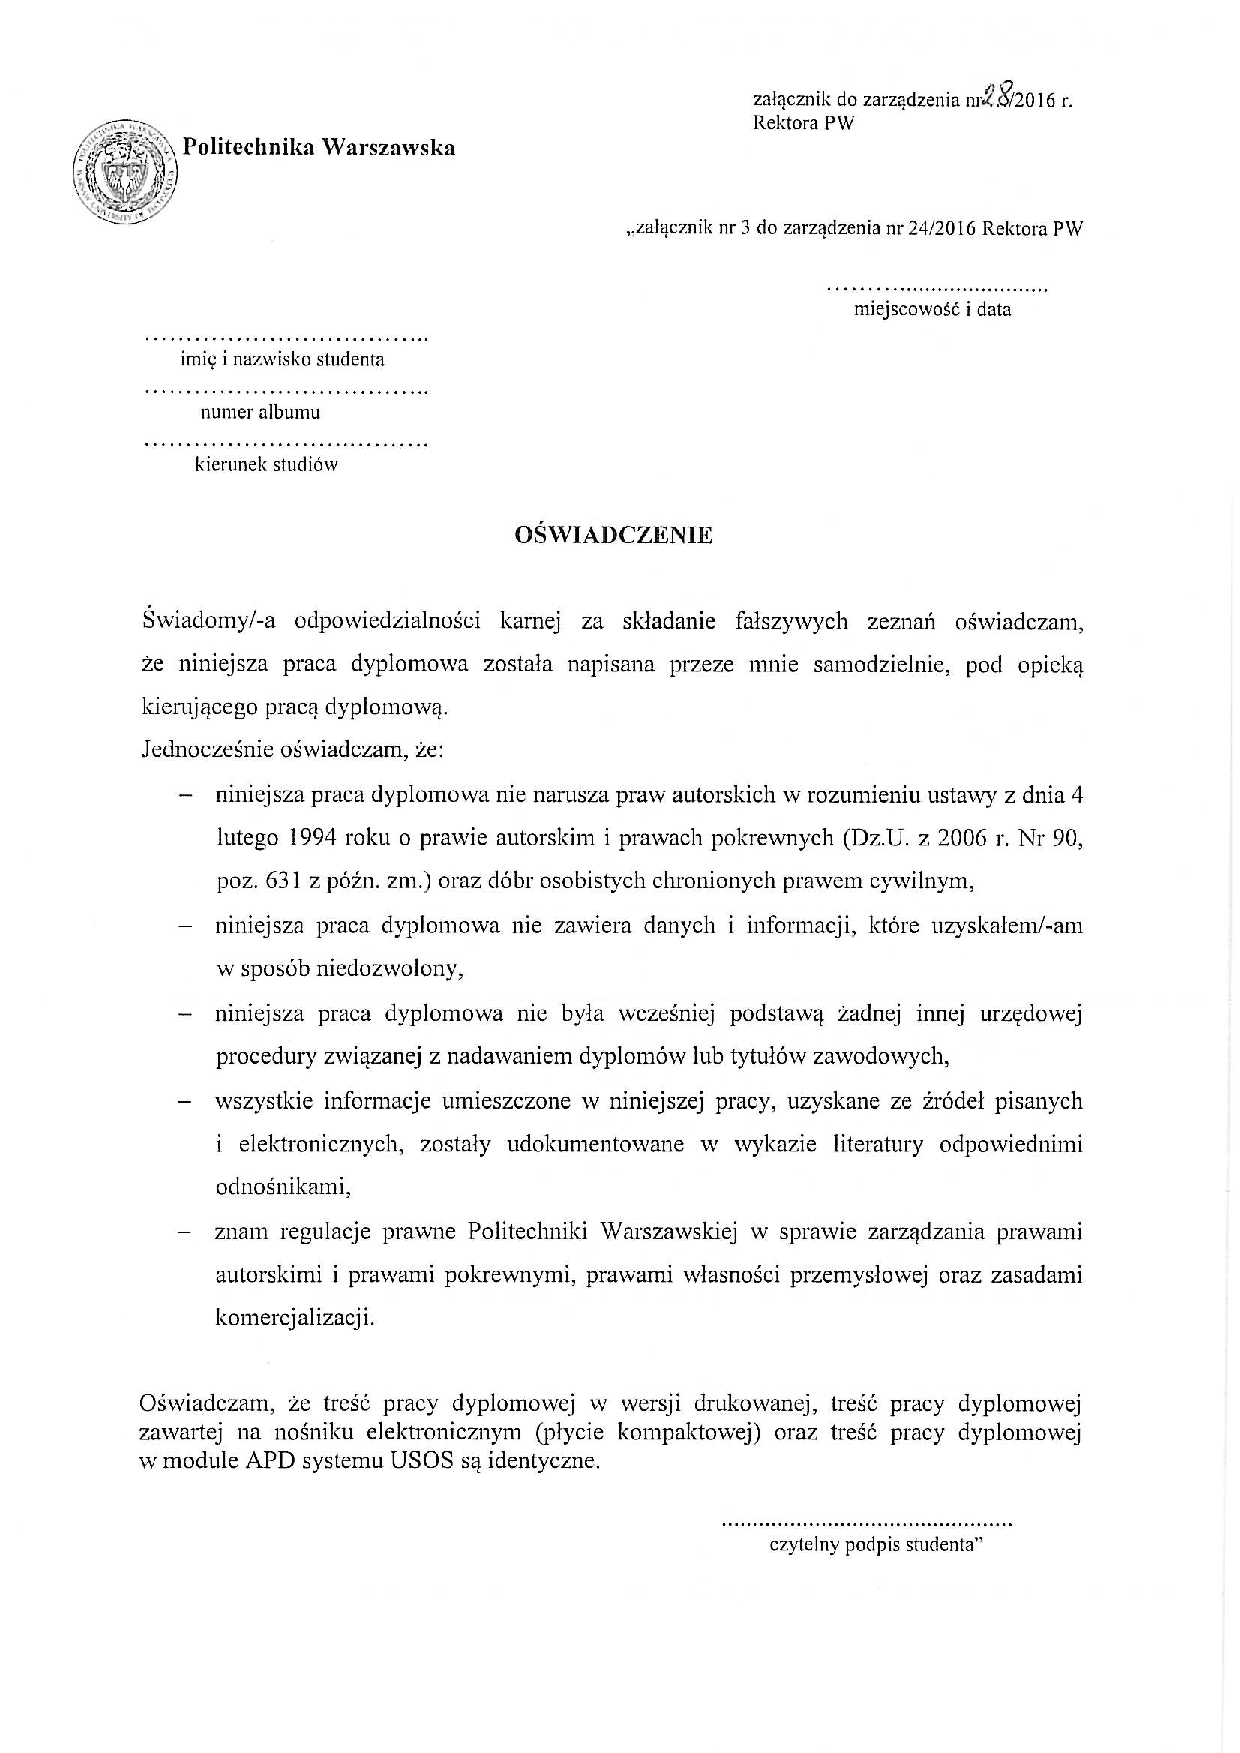
\includepdf[pages=1]{obrazy/oswiadczenie.pdf}
\newpage
\tableofcontents
 
\newpage
\section{Wstęp}  

\subsection{Motywacja}
W dzisiejszych czasach genetyka jest jednym z najważniejszych działów medycyny.
Umiejętność znajdowania natury gnębiących ludzkość chorób
czy to dziedzicznych czy cywilizacyjnych jest jednym z celów obecnie pracujących badaczy. Wczesne wykrywanie chorób u ludzi czy też określenie prawdopodobieństwa 
ich wystąpienia może ocalić wiele istnień. 

Równocześnie z rozwojem technologii umożliwiających tanie i efektywne
pozyskiwanie danych z sekwencjonowania DNA, wzrasta zapotrzebowanie 
na system pozwalajacy na przechowywanie oraz analizowanie zebranych
informacji.
Na świecie istnieje wiele udostępnionych społeczności naukowej baz danych,
z wariantami dziesiątek tysięcy pacjentów. Co za tym idzie powstało 
wiele systemów starających się umożliwić wygodne i efektywne 
przeglądanie oraz analizowanie list wariantów i adnotacji.
Jednak nie udało się stworzyć uniwersalnego narzędzia pozwalającego
wszystkim lekarzom na efektywniejsze i szybsze znajdowanie
genów odpowiedzialnych za choroby czy też mutacje.

Dlatego na Wydziale Elektroniki i Technik Informacyjnych 
oraz w Zakładzie Genetyki Medycznej Instytutu Matki i Dziecka w Warszawie
powstał projekt mający na celu połączyć najnowsze technologie i 
praktyki dotyczące rozproszonych baz danych wraz z wiedzą naukową
lekarzy oraz biologów tak by stworzyć system umożliwiający 
wspomaganie ich codziennej pracy.
  
\subsection{Cel pracy} 
Celem tej pracy inżynierskiej jest stworzenie 
interfejsu użytkownika do opisanej wcześniej 
rozproszonej bazy danych.
Myślą przewodnią projektowania systemu było stworzenie aplikacji 
prezentującej dane z sekwencjonowania DNA użytkownikowi, którą będzie 
można spersonalizować i będzie łatwo konfigurowalna.
Chciano także ograniczyć pracę administratora systemu do
całkowitego minimum i zaimplementować tak strukturę projektu
by rozwijanie go poprzez dodawanie nowych funkcjonalności było
prowadzone niskim kosztem.

Podczas projektowania aplikacji należało zwrócić uwagę na
ilość i rodzaj danych co wymusiło zaprojektowanie specyficznego systemu
filtrującego, w celu umożliwienia ograniczenia widocznych danych
do tylko tych potrzebnych klientowi aplikacji.



\newpage
\section{Specyfika danych}  
Celem zrozumienia osobliwości danych nalezy przedstawic ich pochodzenie 
i znaczenie. Sekwencjonowane są one z z ludzkich genomów, czyli innymi słowy z ludzkiego materiału genetycznego. 

DNA (kwas deoksyrybonukleinowy) to związek organiczny zlokalizowany w jądrach komórkowych. 
Struktura DNA odpowida między innymi za kodowanie białek pełniących w organiźmie wiele ważnych funkcji (np. transpot tlenu między tkankami za co 
odpowiedzialna jest między innymi hemoglobina).

Podstawowymi elementami budującymi nasz kod genetyczny są
nukleotydy. Sposób w jaki są ustawione w sekwencji odpowiada
za ostateczną budowę białka, których sumarycznie ludzkie DNA ma ich około 
600 milionów. Cała ta sekwencja koduje 20-25 tysięcy białek.

Określone miejsce w kodzie genetycznym, koduje określone białko
i w tym miejscu można zaobserwować wiele wariantów (genów), 
które różnią się co najmniej jednym nukleotydem.

Powyższa różnica może spowodować poważne 
zakłócenia w funkcjonowaniu naszego organizmu, a warianty
są elementami, które starają się badać
lekarze poprzez wyszukiwanie tych, które mogą powodować choroby
czy też mutacje.
Podczas budowy białka następuje transkrypcja, czyli przepisanie DNA na RNA
i wynik tej operacji konkretnego wariantu - tak zwany transkrypt był elementem bazy danych używanej przy implementacji systemu.
 
Jeden wiersz w bazie danych (zwana również próbką) stanowi między innymi informacje o:
\begin{itemize}
\item chromosomie owego wariantu,
\item pozycji, na której się różni dany wariant,
\item referencyjnej wartości nukleotydu,
\item wartości nukleotydu, na którą zmienił wariant,
\item częstości występowania tego wariantu,
\end{itemize}



\newpage
\section{Wymagania funkcjonalne i niefunkcjonalne}  

Określenie funkcjonalności dostępnych w budowanej aplikacji, rozpoczęto od określenia 
rodzajów użytkowników, którzy mają korzystać z oprogramowania tak by jak najlepiej dostosować system do ich potrzeb i przyśpieszyć ich pracę.

Pierwszą grupą docelową są lekarze, którzy będą poszukiwali
możliwych chorób powiązanych z wariantem pacjenta, aby wykryć niebezpieczeństwa
i móc jak najwcześniej im przeciwdziałać. 
Dane będą rozpatrywać w kontekście jednego pacjetnta i nalezy umożliwić łatwe rozróznienie genotypów

Drugim grupą są analitycy, którzy będą analizować dane i zadawać 
odwrotne pytania, czyli będą starać się znaleźć warianty, które mogą być odpowiedzialne
za konkretną chorobę. 

Inną istotną kwestią wziętą pod uwagę był typ i wielkość danych, jakie mają być wyświetlane klientom.
W trakcie projektowania architektury jako dane przykładowe zostały wybrane wyniki przykładowego transkryptu dostępne w aplikacji ExAC instututu Broad \cite{exac} \cite{exacCite}. Dane te 
podobnie jak te w rozproszonej bazie danych posiadały ponad 30 kolumn i oczywistym wydało się że obie grupy użytkowników będzie interesowała tylko część informacji o genotypie i należało by umożliwić im filtrację oraz zakrywanie niepotrzebnych danych. 
Jedna próbki z docelowej bazy danych liczą sobie więcej niż 20000 wierszy co wymogło zaproponowanie 
funkcjonalności umożliwiającen na poprawne i intuicyjne ich filtrowanie filtrowanie 
tak aby klient otrzymywał tylko interesujące go rekordy.

\newpage
\subsection{Wymagania funkcjonalne}
Po zakończeniu analizy zostały określone następujące funkcjonalności. Aplikacja:

 \begin{enumerate}[1)]
 \item ma wygodny, prosty interfejs użytkownika,
 \item rejestruje użytkowników,
 \item autoryzuje użytkowników,
 \item umożliwia wybór próbki do analizy,
 \item pozwala na wprowadzenie wcześniej zdefiniowanych filtrów z panelu administratora,
 \item wyświetla dane z sekwencjonowania DNA dla konkretnej próbki,
 \item filtruje dane po stronie serwera i wysła je klientowi,
 \item zlicza ilość danych przy zadanych filtrach i informuje klienta o wyniku,
 \item umożliwia zmianę wartości filtrów,
 \item pozwala na wyłączenie z filtracji dowolnej części filtrów,
 \item zapisuje wartości filtrów oddzielnie dla każdego użytkownika,
 \item sortuje dane po stronie klienta,
 \item filtruje dane po stronie klienta,
 \item udostępnia administratorowi możliwość zmiany dostępu do próbek 
 każdego użytkownika,
 \item daje możliwość zakrycia na stronie aplikacji części danych,	
 \end{enumerate}
 
\newpage

Funkcjonalności umożliwiająca wprowadzanie wcześniej zdefiniowanych filtrów spowodowała stworzenie
specjalnej klasy użytkowników, to jest administratorów, którzy będą zarządzali strukturą filtrów poprzez wprowadzenie odpowiedniego pliku z specjalnie przygotowanego panelu administracyjnego
oraz będą zarządzać dostępem do próbek dla użytkowników.

\subsection{Wymagania niefunkcjonalne}
Aplikacja:
 \begin{enumerate}[1)]
  \item szyfruje wysyłane dane między klientem a serwerem za pomocą protokołu HTTPS,
  \item wykorzystuje funkcję SHA-512 do zabezpieczenia hasła użytkownika,
  \item korzysta z "soli" przy wyliczaniu funkcji skrótu,
  \item wykorzystuje darmowe oprogramowanie,
 \end{enumerate}

\newpage
\section{Istniejące rozwiązania}  

Konieczność posiadania aplikacji umożliwiającej analizę danych z genomów 
jest powszechnie znane od dłuższego czasu. W związku z powyższym 
powstało wiele rozwiązań,
komercyjnych i niekomercyjnych, które starają się sprostać wymaganiom wszystkich użytkowników. W tej sekcji przedstawione zostaną najpopularniejsze opcje.

\paragraph{Ingenuity Variant Analysis} Jednym z wiodących rozwiązań jest aplikacja Ingenuity Variant Analysis \cite{ingenuity} firmy Qiagen. To zaawansowane narzędzie
poza wyświetlaniem danych wariantów, umożliwia między innymi:

\begin{itemize}
\item zaawansowane filtrowanie,
\item eksporty wyników do plików,
\item udostępnienie swojego raportu innemu użytkownikowi,
\end{itemize} 
  
Jest to jednak oprogramowanie komercyjne co wykluczyło go z dalszych 
rozważań.

\begin{figure}[h]
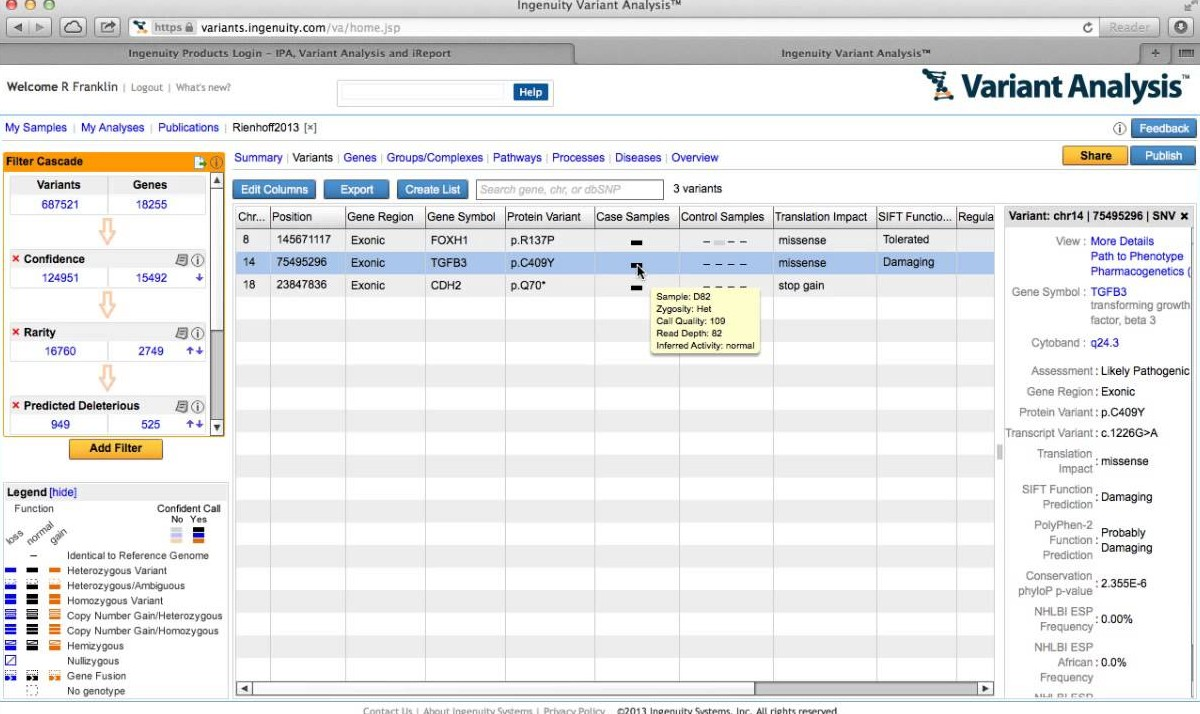
\includegraphics[width=\linewidth]{obrazy/exac/ingenuity.jpg}
  \caption{Ingenuity Variant Analysis \cite{ingenuity}}
  \label{fig:ingenuitypic}
\end{figure}
\newpage

\paragraph{ExAC Browser} ExAC Browser \cite{exac} \cite{exacCite} jest aplikacją, tworzoną przez koalicję badaczy i informatyków, w celu
udostępnienia danych kodujących białka szerszemu gronu badaczy. 
Dokonują tego poprzez harmonizację i agregację danych z wielu projektów.
Jednymi z najmocniejszych zalet aplikacji jest prezentuja dane w postaci tabel, wykresów oraz umożliwianie eksportu danych.
Mimo iż jest to wolne oprogramowanie, nie zdecydowano się na jego wykorzystanie
ponieważ:
\begin{enumerate}[1)]
\item podczas rozważań oprogramowanie było dopiero w wersji beta, 
\item brakowało funkcjonalności filtrowania danych transkryptu,
\item brakowało rozróżnienia użytkowników a to powodowało:
\begin{itemize}
\item brak możliwości personalizacji aplikacji dla użytkownika,
\item brak kontroli nad dostępami do próbek,
\end{itemize}
\end{enumerate}

\begin{figure}[h]
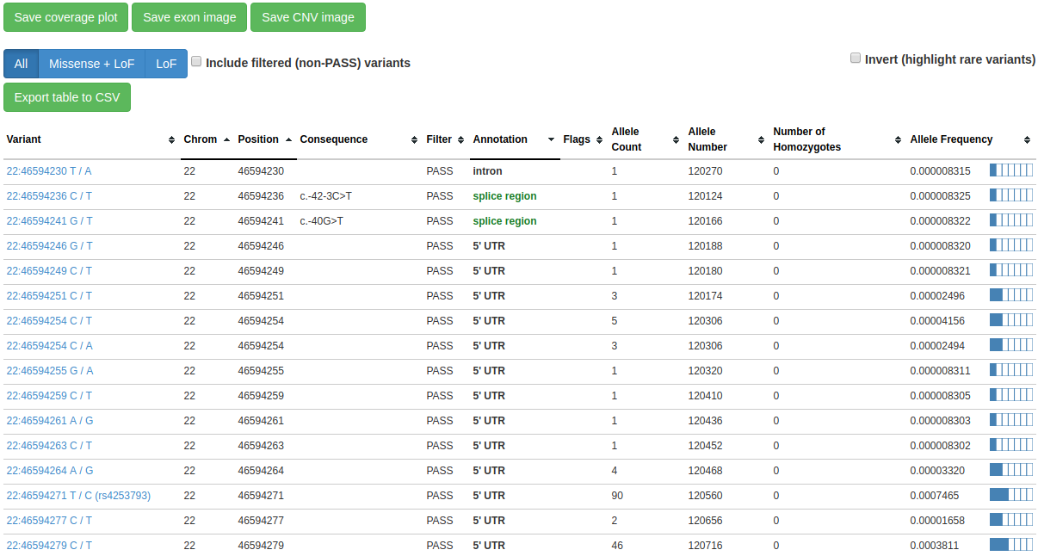
\includegraphics[width=\linewidth]{obrazy/exac/broad.png}
  \caption{Broad}
  \label{fig:broadpic}
\end{figure}

\newpage

\paragraph{VCF-Miner}

Od wielu lat dziesiątki instytucji próbowało stworzyć własne aplikacje do przeglądania danych pochodzących z sekwencjonowania. Zatrzymać to zjawisko
starali się twórcy VCF-Miner'a \cite{miner} \cite{minerArt} poprzez 
stworzenia aplikacji pozwalającej na pracę z próbkami w formacie VCF \cite{vcfformat}. Jest to format pliku tekstowego używanego do przechowywania
danych z sekwencjonowania DNA. 

VCF-Miner'owi mimo swoich wielu zalet takich jak na przykład możliwość
załadowania własnego pliku VCF, braku kilku istotnych z 
punktu widzenia naszych użytkowników funkcjonalności, które zostały 
zostały zaimplementowane w aplikacji, której dotyczy ta praca inżynierska.
Są nimi:
\begin{enumerate}[1)]
\item brak predefiniowanych filtrów, 
\item trudna w obsłudze filtracja danych, to znaczy: 
\begin{itemize}
\item brak możliwości fitracji pobranych już danych,   
\item brak możliwości wyłączenia jednego filtru bez usuwania go w całości,
\item możliwość usunięcia tylko ostatniego w kolejce filtru,
\end{itemize}
\item brak zapisu ukrytych kolumn - użytkownik przy każdej próbce
musi ponownie ukrywać bądź odsłaniać interesujące go kolumny,
\item brak ograniczanie dostępu do próbek - każdy użytkownik ma dostęp
do wszystkich próbek,
\end{enumerate}

\begin{figure}[h]
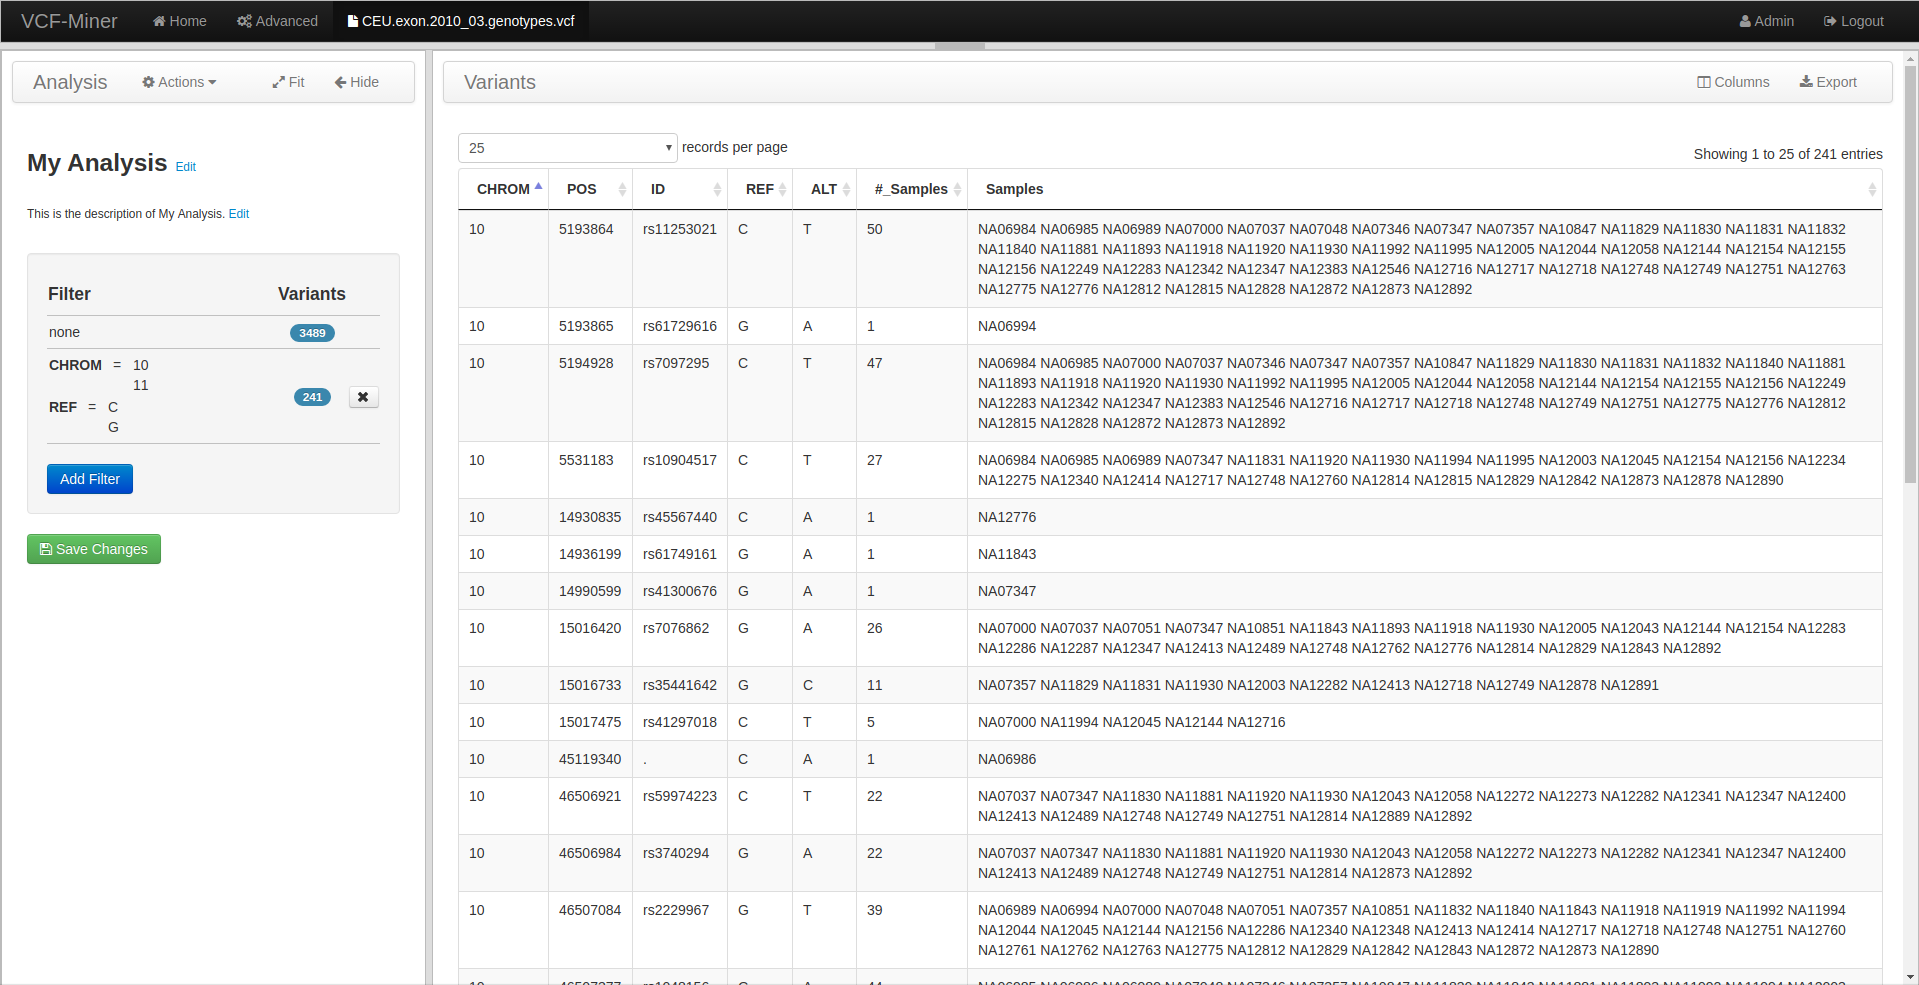
\includegraphics[width=\linewidth]{obrazy/exac/miner.png}
  \caption{Miner}
  \label{fig:minerpic}
\end{figure}


\newpage
\section{Wybór technologi}

Platforma klastrowego przetwarzania danych - Apache Spark\cite{spark}, z którą współpracować będzie aplikacja, została stworzona oraz udostępnia interfejs programistyczny w języku Scala.
Naturalnym przez to wydało się wybranie tego języka programowania do stworzenia przeglądarki danych.

  
\subsection{Język programowania Scala}
W aplikacji użyto języka Scala w wersji 2.11.7 \cite{jezykScala}. Jest to język programowania powstały w 2001 roku pod kierownictwem Martina Odersky'ego w Lozannie.
Działa na Wirtualnej Maszynie Javy a do 2012 roku wspierała platformę .NET opracowaną przez firmę Microsoft. 

Język ten nadaje się równie dobrze do krótkich, zwartych skryptów  wywoływanych podobnie do skryptów języka Python jak i do tworzenia wydajnych, ogromnych, bezpiecznych systemów sieciowych.
Jest językiem łączącym cechy języków funkcyjnych oraz obiektowych. 
Nie jest jednak obligatoryjny funkcyjny styl programowania, do którego nie jest przyzwyczajona większość programistów.

 Scala w swoim założeniu nawiązuje do minimalizmu składni Lispa to znaczy że nie opiera się na składni ale na funkcjach bibliotecznych. Nazwa ma podkreślić skalowalność języka, dzieje się tak dzięki możliwości tworzenia dodatkowych typów i struktur wyglądających jak nowa składnia języka.
Zaletą języka jest również to że dzięki kompatybilności z językiem Java mamy możliwość wykorzystania każdej lini kodu napisanej w owym języku.

\subsection{System zarządzania bazą danych}  
Zadanie stworzenia bazy danych przechowującej informacje konfiguracyjne, dane użytkowników oraz o użytkownikach było dużą częścią tworzenia systemu i
wymagało wybrania odpowiedniego systemu zarządania bazą danych.
Model bazodanowy został zaprojektowany w modelu opartym na relacyjnej organizacji danych, przez co wybór ograniczył się do
darmowych technologii realizujących relacyjne bazy danych.

Biorąc pod uwagę powyższe kryteria, można porównać najpopularniejsze systemami, są nimi\cite{porownanieBaz}: 
 \begin{itemize}
  \item MqSQL,
  \item SQLite,
  \item PostgreSQL,
\end{itemize}

\subsubsection{MySQL}
\paragraph{Zalety}
\begin{itemize}
\item{proste i łatwe w obsłudze},
\item{wysoki poziom bezpieczeństwa},
\end{itemize}
\paragraph{Wady}
\begin{itemize}
\item{nie realizuje w pełni standardu SQL},
\item{problematyczny jednoczesny zapis i odczyt},
\end{itemize}
\subsubsection{SQLite}
\paragraph{Zalety}
\begin{itemize}
\item{zgodny ze standardem SQL},
\item{przenośny dzięki oparciu bazy o jeden plik},
\end{itemize}
\paragraph{Wady}
\begin{itemize}
\item{brak zarządzania użytkownikami i dostępami do danych},
\end{itemize}

\subsubsection{PostgreSQL}
\paragraph{Zalety}
\begin{itemize}
\item{zgodny ze standardem SQL},
\item{wsparcie dla współbieżności},
\item{pełne wsparcie dla transakcji},
\end{itemize}
\paragraph{Wady}
\begin{itemize}
\item{słaba wydajność},
\item{trudność instalacji dla początkujących użytkowników},
\end{itemize}

\subsubsection{Uzasadnienie wyboru PostgreSQL}
Po analizie ostateczny wybór systemem padł na PostgreSQL.
To otwarte i darmowe oprogramowanie posiada bardzo dużą społeczność, której wiedza jest łatwo dostępna w internecie 
i posiada wiele narzędzi i bibliotek przeznaczonych do pracy z owym systemem. 
Istotny wpływ na decyzje miała również łatwość integracji PostgreSQL na inne systemy.  

\subsection{Slick}  
Pracę z bazą danych po stronie serwera aplikacyjnego 
znacznie ułatwia oprogramowanie pozwalające na odwzorowanie obiektowo-relacyjne tabel bazodanowych na obiekty języka programowania.
Dzięki tej technice programista może traktować obiekty bazodanowe jak elementy kolekcji czy pola obiektów.

Takim narzędziem jest stworzone przez firmę Lightbend, Inc. 
oprogramowanie Slick\cite{slick} pozwalające na pełną kontrolę nad bazą danych oraz pisanie klasycznych zapytań SQL.

\subsection{JDBC}  
Baza danych zawierająca dane o sekwencjonowaniu DNA jest kolumnowo zorientowaną bazą danych opartą na systemie Apache Kudu \cite{kudu}. W przeciwieńswie do tradycyjnych systemów bazodanowych gdzie dane składowane są poziomo czyli wierszami, w kolumnowych systemach dane przechowywane są pionowo - kolumnami.
Kudu zajmuje się składowaniem danych, za wykonywanie zapytań SQL 
odpowiada całkowicie zintegrowane z Kudu oprogramowanie Impala \cite{impala} \cite{impalaArt} udostępniająca interfejs JDBC.

\subsection{Aplikacja przeglądarkowa}
Biorąc pod uwagę wymagania klientów oraz różnorodność używanych przez nich urządzeń należało wybrać odpowiedni rodzaj aplikacji klienckiej pozwalający na spełnienie wszystkich wymagań funkcjonalnych naszych użytkowników 
oraz jednocześnie będący łatwy w utrzymaniu i rozwijaniu.

\paragraph{Zalety aplikacji internetowych}
Łatwość w dostępie do internetu i ilość urządzeń pozwalających na 
korzystanie z przeglądarek internetowych pozwoliły 
na rozwój aplikacji internetowych oraz ich rozpowrzechnienie.
Łatwość w rozbudowie, zarządzaniu i 
niskie ceny wynajmowania serwera aplikacyjnego spowodowały 
powstanie grupy platform programistycznych wspomagających ich budowę. 

Narzędzia typu Ruby on Rails czy Spring Boot 
zdejmują z programisty obowiązek konfiguracji serwera 
HTTP od podstaw i umożliwiają rozpoczęcie pracy  
nad stronami aplikacji po kilku minutach.

\paragraph{Platforma programistyczna Play}
Platforma Play, stworzona w języku Scala jest środowiskiem 
do tworzenia aplikacji internetowych, 
która na celu ma przyśpieszyć pracę programisty dzięki:
\begin{itemize}
\item strategii Konwencji Ponad Konfigurację,
\item przeładowywania i ponownej kompilacji plików po edycji,
\item wykorzystaniu wzorca Model-Widok-Kontroler,
\item wykorzystaniu technologii REST,
\end{itemize} 
  
\paragraph{Platforma programistyczna Angular}
Angular jest opracowaną przez Google biblioteką wspomagającą tworzenie 
aplikacji przeglądarkowych na jednej stronie. Jej głównymi zaletami jest :
\begin{itemize}
\item odzielenie warstwy klienckiej od warstwy serwerowej,
\item oddzielenie manipulacji modelu dokumentu HTML od logiki aplikacji,
\item wykorzystaniu wzorca Model-Widok-Kontroler,
\end{itemize} 
    
\paragraph{Lodash} Biblioteka Lodash \cite{lodash} jest zbiorem wielu użytecznych funkcji ułatwiających pracę z typami dostępnymi w języku Javascript. 
  
\newpage
\section{Przypadki użycia}
\subsection{Autoryzacja} 
\subsubsection{Role}
Administratorem nazywana jest osoba mająca dostęp do bazy danych aplikacji, ustalająca
widoczne dla użytkowników próbki oraz zarządzająca strukturą filtrów. 
Jednocześnie administrator ma takie same możliwości jak zwykły użytkownik, którymi są dostęp do określonych próbek, możliwość ich oglądania, filtrowania i  ukrywania kolumn. 
Każdy użytkownik jest rozróżnialny w aplikacji dlatego wymagana jest wcześniejsza rejestracja.
 
\subsubsection{Rejestracja i logowanie użytkownika}
Poniższy rysunek pokazuje widok startowy aplikacji. W celu przejścia do 
pozostałych funkcjonalności, użytkownik musi się zalogować lub zarejestrować, jeśli nie ma jeszcze 
konta w aplikacji. Wskazane jest użycie szyfrowanego połączenia HTTPS, żeby uniknąć 
kradzieży hasła.

\begin{figure}[h!]
  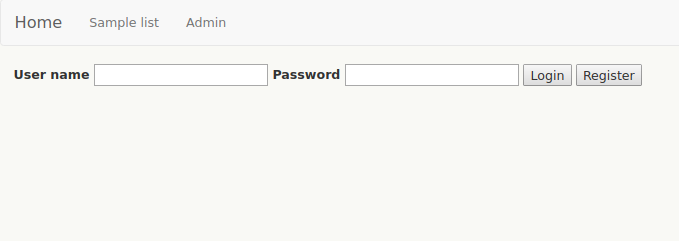
\includegraphics[width=\linewidth]{obrazy/aplikacja/login.png}
  \caption{Okno logowania i rejestracji}
  \label{fig:loginpic}
\end{figure}

\newpage  
\subsection{Przeglądanie danych z sekwencjownowania DNA} \label{sssec:dnaPage}
Po zalogowaniu się do aplikacji przed użytkownikiem pojawia się główna część aplikacji pozwalająca na dostęp do próbek oraz pracę na nich. 
 
\paragraph{Ekran dostępnych genomów}
Każda próbka dostępna w bazie danych posiada indywidualny identyfikator pozwalający na 
rozróżnienie jej od innych próbek. Owy identyfikator jest ciągiem znaków, który wyświetlany jest 
alfabetycznie posortowanej liście. Użytkownik widzi tylko próbki udostępnione przez administratora
i ma możliwość spojrzenia dokładniej w dane poprzez kliknięcie w identyfikator próbki,
co przeniesie go do następnej strony prezentującej dane z sekwencjonowania DNA. 


\begin{figure}[h!]
  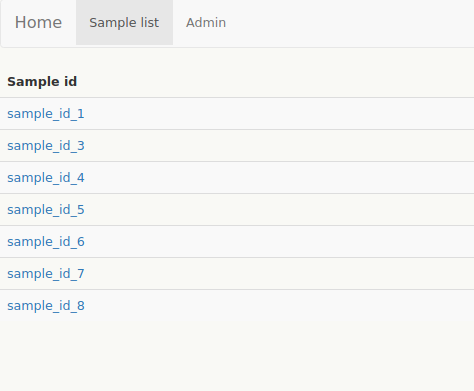
\includegraphics[width=\linewidth]{obrazy/aplikacja/sample_list.png}
  \caption{Lista próbek}
  \label{fig:sample_listpic}
\end{figure}

\newpage
\paragraph{Tabela z danymi z sekwencjonowania DNA} 
Przechodzą na stronę z danymi dla konkretnej próbki, użytkownikowi prezentowane są 
dane w postaci tabelarycznej (Rysunek numer \ref{fig:table1pic}).

\begin{figure}[h!]
  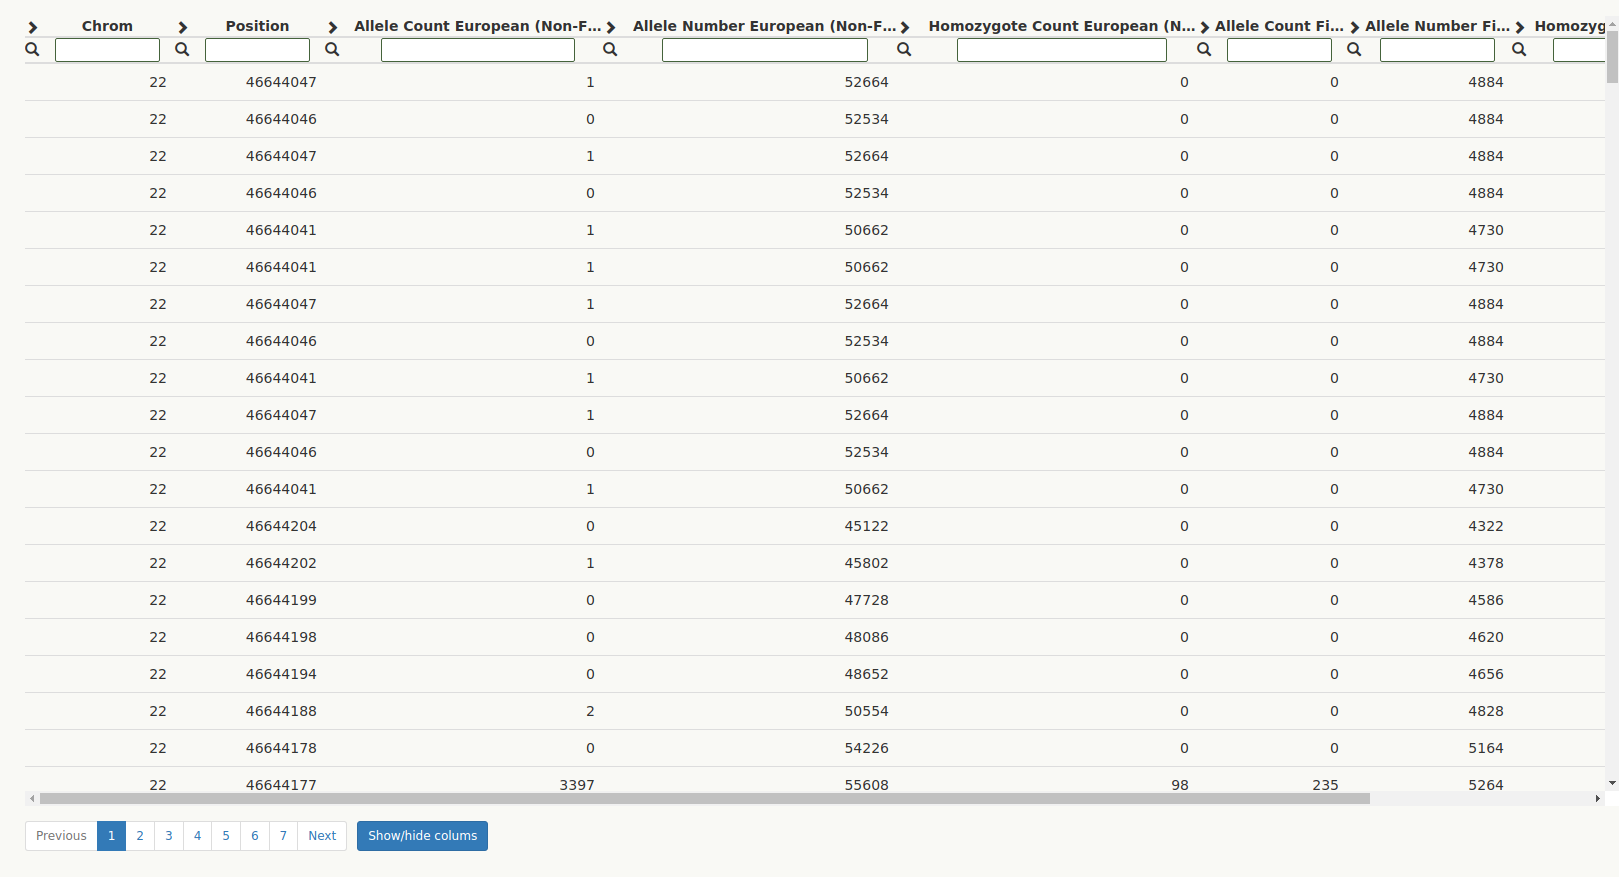
\includegraphics[width=\linewidth]{obrazy/aplikacja/table1.png}
  \caption{Tabela z danymi z sekwencjonowania DNA}
  \label{fig:table1pic}
\end{figure}

Po zakończeniu implementacji wyświetlania tabeli z danymi z sekwencjonowania DNA,
zauważono problemy z wydajnością.
Długi czas tworzenia się elementów HTML tabeli i łatwo zauważalne zawieszanie się przeglądarki
były elementami nie do przyjęcia dla codziennej pracy użytkownika.
Pod obserwację wzięto:
\begin{itemize}
\item czas odpowiedzi serwera na zapytanie HTTP,
\item czas wygenerowania i wykonania zapytania SQL,
\item czas wygenerowania przez przeglądarkę elementów HTML tabeli,
\end{itemize} 
Wykonane testy wykazały, że największy narzut czasowy na ładowanie się strony, miał ostatni 
element to znaczy rysowanie tabeli przez przeglądarkę. 

Wada ta została zniwelowana poprzez wprowadzenie paginacji zwanej też stronicowaniem.
Maksymalna ilość pokazywanych wierszy została ograniczona do 300 i wprowadzono dodatkowy 
element widoczny w lewym dolnym rogu rysunku numer \ref{fig:table1pic}, który umożliwia 
użytkownikowi poruszanie się po kolejnych stronach tabelki zmniejszając narzut 
pamięci operacyjnej wymaganej do wygenerowania całości tabeli.  
\newline

Ważną funkcjonalnością z punktu widzenia użytkownika jest możliwość filtracji pobranych już wierszy
z bazy danych. W celu zwiększenia możliwości wyszukiwania, każda kolumna posiada oddzielne pole 
filtrujące, umożliwiając na zawężanie zbioru danych po każdej kolumnie. Element odpowiadający
za stronicowanie poprawnie zmniejsza ilość dostępnych stron przy dynamicznym zmniejszaniu się
wyświetlanych danych.
Dodatkową opcją działającą po stronie przeglądarki jest 
funkcjonalność sortowania rosnąco bądź malejąco jednej kolumny. Służy do tego strzałka po
lewej stronie od nazwy kolumny, kliknięcie w ikonkę bądź nazwę kolumny zmienia sortowanie.

\begin{figure}[h]
\centering
  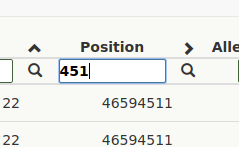
\includegraphics{obrazy/aplikacja/sortingAndSearch.png}
  \caption{Sortowanie i filtrowanie pobranych już danych}
  \label{fig:sortingAndSearchpic}
\end{figure}

\newpage
\paragraph{Ustawianie widoczności kolumn}
Przejżystość danych i dostęp tylko do potrzebnych informacji jest kluczową wartością dla użytkowników.
Mnogość kolumn, porowadząca do przedstawianie wielu informacji niepotrzebnych 
wszystkim użytkownikom uniemożliwia osiągnięcie tego efektu. Wychodząc naprzeciw tym oczekiwaniom 
zaimlementowano opcję umożliwiającą klientom aplikacji ukrywanie dowolnej kolumny.
Po kliknięciu w specjalny guzik umiejscowiony po prawej stronie elmentu stronicującego, wyskakuje okienko z listą kolumn,
które użytkownik może odznaczyć co spowoduje zniknięcie z tabeli. Selekcja może być zapisana 
w bazie danych tak by przy ponownym wejściu na tą stronę aplikacji, użytkownik nie musiał
kolejny raz ukrywać nieinteresujących go kolumn. Po rejestracji użytkownik ma widoczne wszystkie
kolumny i musi sam je odznaczyć.

\begin{figure}[h]
  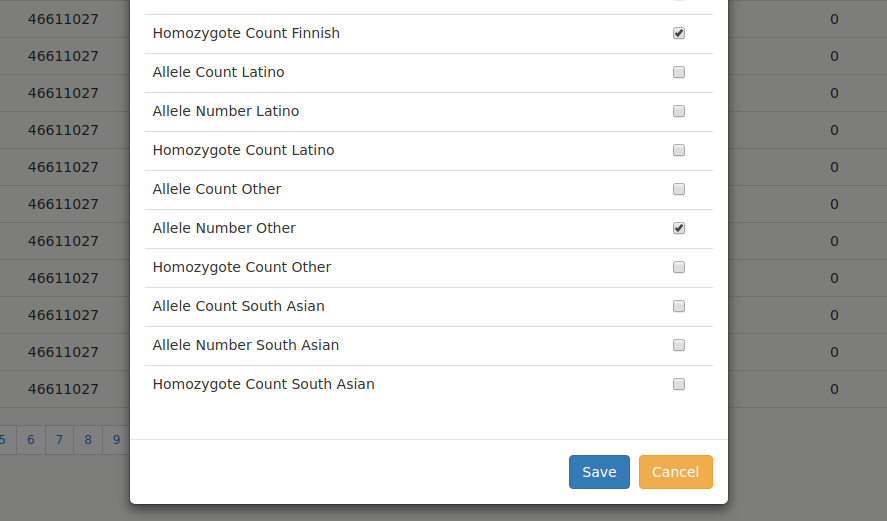
\includegraphics[width=\linewidth]{obrazy/aplikacja/visible_columns.png}
  \caption{Widoczne kolumny}
  \label{fig:visible_columnspic}
\end{figure}

\newpage
\paragraph{Filtrowanie danych}
Rysunek numer \ref{fig:filterspic} przedstawia moduł filtrujący dane, znajdujący się w
lewej części strony aplikacji.
Podstawowym elementem tworzącym filtr jest tak zwane "pole", odnosi się ono do jednej kolumny
bazodanowej, z którą łączy ją jedna z poniższych relacji: 

\begin{itemize}
\item mniejsze (less),
\item większe (greater),
\item mniejsze równe (less than),
\item większe równe (greater than),
\item równe (equals),
\end{itemize} 

Użytkownik wprowadza własną wartość do pola bądź wybiera ją z listy rozwijanej.   
Dodatkową możliwością jest pole mające wartość domyślną ustaloną przez administratora. 
Wartość każdego pola może być zapisane w bazie danych, zapis jest oddzielny, dla każdego 
użytkownika, każdego filtru oraz każdej próbki.
Grupa pól tworzy właściwy "filtr", który może być wyłączony z filtracji dzięki
przyciskowi wyboru z etykietą "Inactive". Wizualnie filtr jest wyciemniony jak na przykładzie.
Grupa filtrów tworzą tak zwany panel, które są oddzielnymi bytami w bazie danych, o własnych nazwach i filtrach.
W górnej części panelu widoczne są przyciski z nazwami paneli. Aktywny panel
wyróżnia się od zielonym kolorem od nieaktywnych o kolorze szarym. 

\begin{figure}
  \centering
  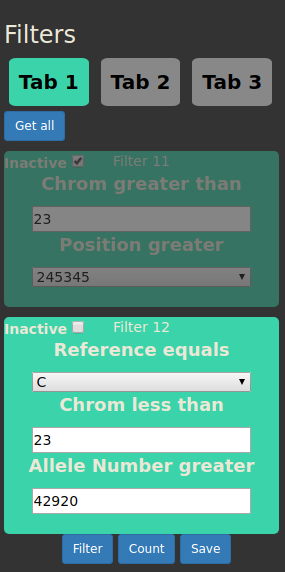
\includegraphics{obrazy/aplikacja/filters.png}
  \caption{Filtry}
  \label{fig:filterspic}
\end{figure}

\newpage

Filtrowanie odbywa się zgodnie z kolejnością aktywnych filtrów, to znaczy najpierw filtrujemy
dane używając pól pierwszego aktywnego filtru, następnie te dane filtrujemy korzystając z drugiego etc. Ilustruje to przykład z rysunku numer \ref{fig:countpic}. Pierwszy filtr o nazwie "Filter 11" redukuje listę wyświetlanych wierszy do 20224. Była by to liczba widocznych wierszy przy deaktywacji pozostałych filtrów. Filtr "Filter 11" razem z drugim filtrem o nazwie "Filter 12"
redukuja liczbę rekordów do 7424

Przycisk z etykietą "Count" umożliwia policzenie ilości wierszy zwróconych przy zadanych wartościach pól. Pozwala to na sprawdzenie rozmiaru danych przed właściwym pobraniem całego zbioru danych.

Można również pobrać wszystkie dane wybranej próbki za pomocą guzika z napisem "Get all".

Za ustalanie struktury filtrów odpowiadają administratorzy i w podrozdziale im poświęconym
opisane zostanie zarządzanie filtrami.


\begin{figure}
  \centering
  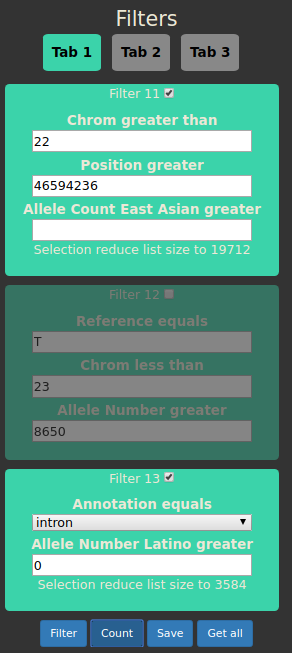
\includegraphics{obrazy/aplikacja/count.png}
  \caption{Wynik zliczania danych}
  \label{fig:countpic}
\end{figure}

\newpage
\subsection{Panel administratora}
Użytkownik o roli administratora może wejść do oddzielnej strony aplikacji (rysunek \ref{fig:adminpic}). Administratorowi prezentowana jest lista zarejestrowanych użytkowników wraz z ich rolami. Każdy element list jest hiperłączem prowadzącym
do strony poświęconej konkretnemu użytkownikowi i jego uprawnieniom.

Przycisk o etykiecie "Upload" służy administratorowi do zmiany struktury 
filtrów, o czym będzie mowa w następnym paragrafie.


\begin{figure}[h]
  \centering
  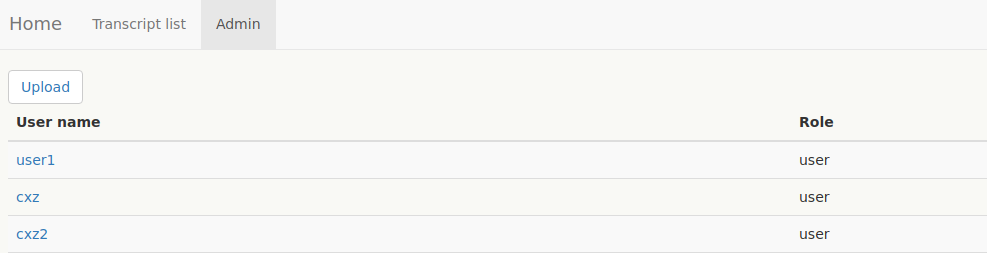
\includegraphics[width=\textwidth]{obrazy/aplikacja/admin.png}
  \caption{Część panelu administratora z listą użytkowników}
  \label{fig:adminpic}
\end{figure}

\newpage
\paragraph{Zarządzanie filtrami}

Zmiana struktury filtrów odbywa się z panelu administratora poprzez wysłanie
z przeglądarki na serwer plik arkusza kalkulacyjnego o ustalonym formacie. Przykładowe dane są widoczne na rysunku \ref{fig:input_filepic}.
W pierwszej kolumnie podaje się nazwę panelu, do której przypisywany
jest filtr o nazwie podanej w drugiej kolumnie. W trzeciej kolumnie należy podać nazwę kolumny, do której
odnosić się będzie pole filtru a następnie relację między wprowadzaną wartością a kolumną.
Opcjonalnie może być podana domyślna wartość pola oraz kilka wartości odzielone przecinkami, między którymi użytkownik będzie mógł wybierać w aplikacji. Nazwy kolumn oraz relacje zostały są dostępne pod
listą rozwijaną w arkuszu w celu ułatwienia pracy administratora. 
Załadowanie pliku usuwa wcześniejsze filtry oraz zapisane wartości użytkowników. 
 
\begin{figure}[h!]
  \centering
  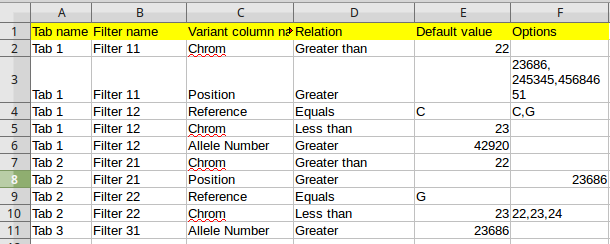
\includegraphics[width=\textwidth]{obrazy/aplikacja/input_file.png}
  \caption{Przykładowa zawartość pliku konfiguracyjnego dla filtrów}
  \label{fig:input_filepic}
\end{figure}

\newpage
\paragraph{Zarządzanie widocznością próbek dla użytkowników}
Po wybraniu użytkownika z listy widocznej na rysuknu numer \ref{fig:adminpic}, 
administratorowi ukazuje się lista wszystkich dostępnych próbek (rysunek numer \ref{fig:user_priviligespic}). Administrator zaznacza w przyciskach wyboru, które próbki będą dostępne 
do wglądu wybranemu użytkownikowi. By zatwierdzić wybór należy kliknąć w 
przycisk z etykietą "Save".
Po zarejestrowaniu się do aplikacji, użytkownik nie jest przypisany do żadnej próbki. 
 
\begin{figure}[h]
  \centering
  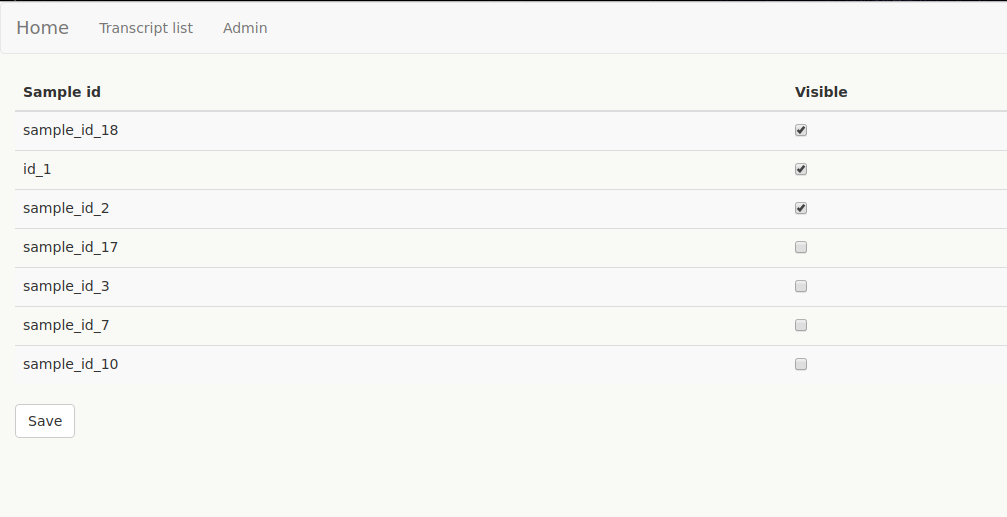
\includegraphics[width=\textwidth]{obrazy/aplikacja/user_priviliges.png}
  \caption{Panel dostępności próbek dla użytkownika}
  \label{fig:user_priviligespic}
\end{figure}

\newpage
\newgeometry{left=0.5cm,bottom=0.5cm, right=0.5cm, top=0.5cm}
\section{Schemat bazy danych}
\begin{figure}[h!]
  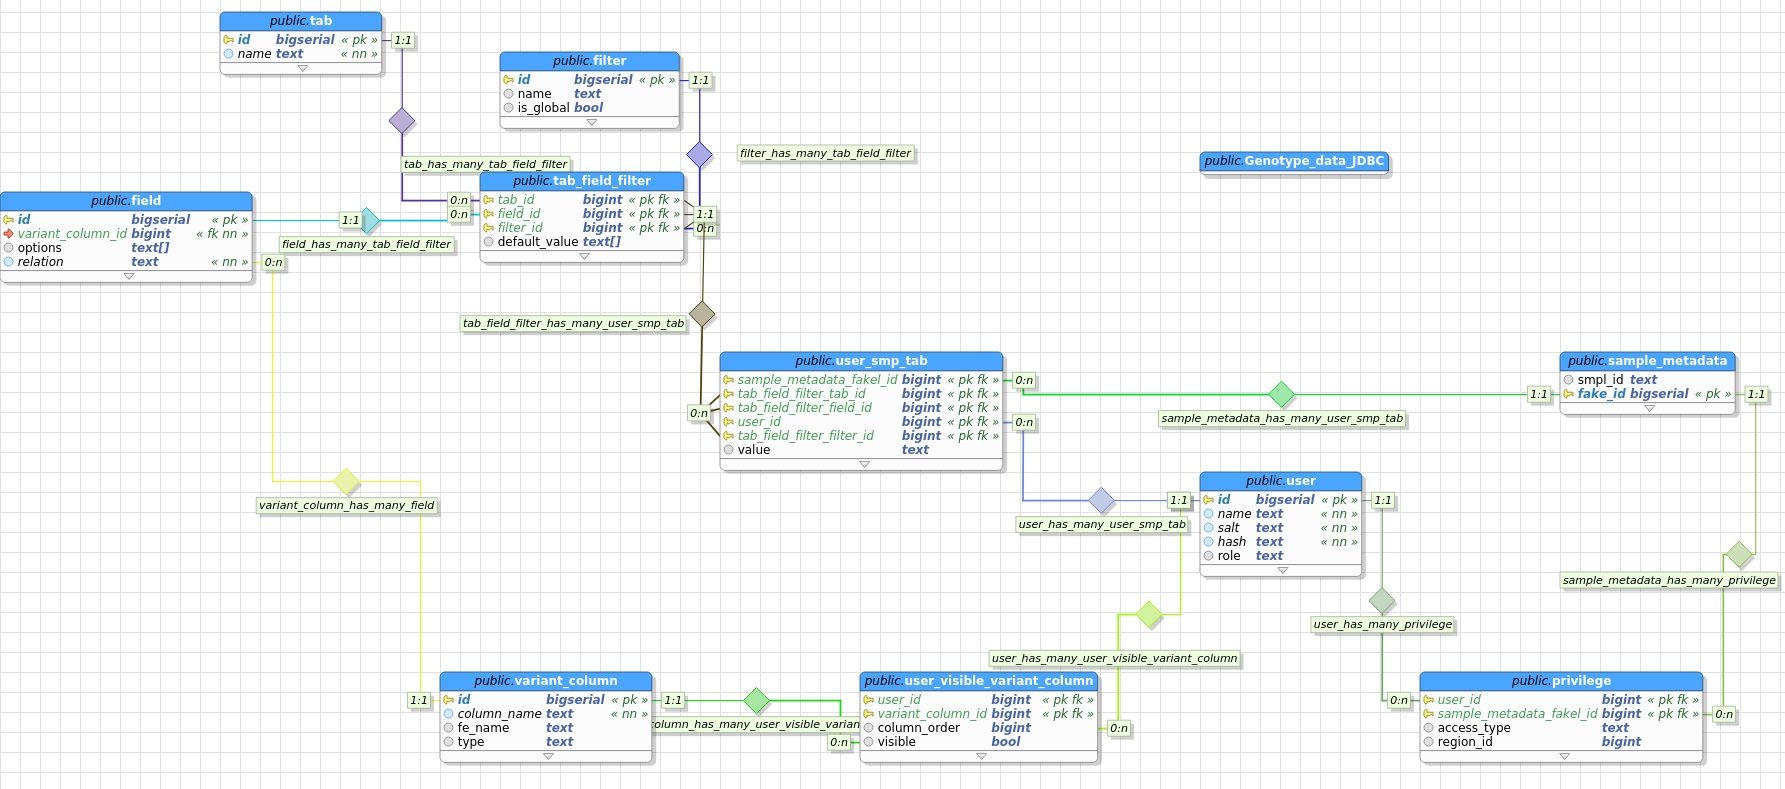
\includegraphics[width=\textwidth, height=0.9\textheight]{obrazy/aplikacja/database.png}
  \caption{Schamat bazy danych}
  \label{fig:bazadanych}
\end{figure}

\restoregeometry
\newpage

Przed rozpoczęciem implementacji aplikacji przeglądarkowej zaprojektowano strukturę 
relacyjnej bazy danych. Na rysunku nr \ref{fig:bazadanych} przedstawiono schemat stworzony
w narzędziu pgModeler \cite{pgModeler}. Dzięki temu darmowemu narzędziu wygenerowany został
skrypt tworzący bazę danych.  

\paragraph{Dane o użytkowniku} Tabela "user" zawiera rekordy o użytkownikach. 
Są to:
\begin{enumerate}[1)]
\item nazwy jakie wybrali przy rejestracji i jakimi posługują się w aplikacji ("name"),
\item role jaką przydzielili im administratorzy systemu ("role"),
\item sól użytą do wygenerowania skrótu i potrzebną do autoryzacji ("salt"),
\item wynik funkcji skrótu z ich hasła ("hash"),
\end{enumerate}

\paragraph{Dane z sekwencjonowania DNA} Podczas trwania okresu implementacji systemu,
przykładowe dane z serwisu Exac zostały załadowane do oddzielnej tabeli bazodanowej o nazwie "Genotype\verb!_!data\verb!_!JDBC". Mimo, iż owa tabela znajdowała się w tej samej bazie danych co 
dane o filtrach czy użytkownikach, aplikacja łączyła się oddzielnym połączeniem. 
Dodatkowo do pobierania danych wykorzystywała interfejs JDBC, tak by jak najlepiej
symulować produkcyjne połączenie aplikacji, czyli połączenie do rozproszonej bazy danych.

\paragraph{Sztuczne identyfikatory próbek} Do implementacji strony
prezentującej dane użytkownikowi (podrozdział \ref{sssec:dnaPage}) planowano użyć 
funkcjonalności platformy Angular, umożliwiającej przekazywanie parametrów 
poprzez część adresu URL. Rozróżnianie próbek odbywa się względem ich nazw, które
są dowolnymi ciągami znaków. Biorąc pod uwagę konieczność zabezpieczenia aplikacji przed 
znakami specjalnymi, które mogłyby się pojawić w nazwie oraz potrzebę
użycia identyfikatora próbki jako klucza obcego w części tabel systemu, postanowiono
dodać dodatkową liczbową kolumnę ("fake\verb!_!id"), której wykorzystanie ułatwiło implementację systemu.

\paragraph{Dostęp do próbek} W tabela "privilege" przechowywane są informacje o 
dostępie użytkownika do danej próbki. Brak rekordu wiążącego użytkownika z 
daną próbką jest w aplikacji rozumiany jako brak dostępu do danej próbki,
przez co po zarejestrowaniu się użytkownika, nie ma On dostępu do żadnej próbki,

\paragraph{Lista kolumn} System był projektowany z myślą by ograniczyć w przyszłości konieczność zmian 
w kodzie aplikacji i by był konfigurowalny z jednego pliku dostępnego administratorowi.
Z tym przeświadczeniem została dodana tabela "variant\verb!_!column", która będzie zawierać
informacje o kolumnach tabeli z danymi DNA. Poza nazwami tych kolumn, które będą 
wykorzystywane do generowania zapytać pobierających dane, w tej encji znajdują
się nazwy wyświetlające się użytkownikowi aplikacji ("fe\verb!_!name") oraz informacje o typach
tych kolumn, służące do sprawdzania poprawności danych wejściowych od klientów.

\paragraph{Widoczność kolumn} Za składowanie informacji o widocznych kolumnach na
stronie prezentującej użytkownikowi dane o sekwencjonowaniu, odpowiada tabela \newline
"user\verb!_!visible\verb!_!variant\verb!_!column". Zapisane w niej są:
\begin{enumerate}[1)]
\item identyfikator użytkownika ("user\verb!_!id"),
\item identyfikator kolumny wariantu ("variant\verb!_!column\verb!_!id"),
\item dana typu boolowskiego ("visible") informująca o widoczności kolumny w następujący sposób:
\begin{itemize}
\item prawda - kolumna jest widoczna,
\item fałsz - kolumna nie jest widoczna,
\end{itemize}
\end{enumerate} 

\newpage
\paragraph{Przechowywanie schematu filtrów} W trakcie analizy wymagań i projektowaniu systemu wydzielono trzy odzielne obiekty tworzące moduł filtrujące dane, to znaczy panele, filtry i pola.
Ułatwiło to zaprojektowanie odpowiednich encji bazodanowych.

Tabela odpowiadająca panelowi ("tab") poza identyfikatorem ("id") przechowuje również unikalną nazwę ("name") widoczną w górnej części panelu filtrującego. 
Podobnie skonstruowana jest encja odpowiadająca jednemu filtrowi ("filter") z tą różnicą, 
iż nazwa ("name") nie jest unikalna. 

Encja będąca odpowiednikiem jednego pola ("field") również została dodana do schematu bazy danych,
z następującymi kolumnami: 
\begin{enumerate}[1)]
\item identyfikator ("id"),
\item identyfikator kolumny wariantu ("variant\verb!_!column\verb!_!id"), powiązanej z polem,
\item relacja między polem a kolumną wariantu,
\item opcjonalne wartości ukazywane użytkownikowi pod listą rozwijaną,
\end{enumerate}

Za łączenie wszystkich trzech wymienionych encji, odpowiada tabela 
"tab\verb!_!field\verb!_!filter", posiadająca identyfikatory każdej z encji oraz
domyślne wartości zadeklarowane przez administratora.

\paragraph{Zapisywanie wartości filtrów dla użytkownika} 
Ostatnią zaprojektowaną tabelą jest tabela "user\verb!_!smp\verb!_!tab",
\textcolor{red}{
 zmienić nazwę, niezgodna z nazewnictwem reszty tabel
}
Funkcjonalność zapisania wartości dla każdego pola filtru, oddzielnie dla każdej próbki
jest zrealizowana poprzez przechowywanie identyfikatora panelu, filtru i pola elementu filtracji,
razen z identyfikatorem próbki i wybraną wartością. 

\newpage
\section{Wydajność aplikacji}  

Dane używane podczas implementacji do sprawdzenia działania aplikacji pochodziły
z Instututu Broad.
Do testów wybrano transkrypt ENST00000407236 \cite{testData},
którego dane były dostępne w pliku CSV. Rozmiar danych wynosił 530 wierszy, każdy posiadający 37 atrybutów. Plik został załadowany do lokalnej bazy danych, do tabeli 
"Genotype\verb!_!data\verb!_!JDBC". Należy zaznaczyć, iż spodziewana ilość wierszy dla jednej próbki wynosi około 20000.
 W celu sprawdzenia zachowania się aplikacji 
dla większych rozmiarów danych, postanowiono kilkakrotnie zmultiplikować
ilość wierszy i zapisać je jako oddzielne próbki.

Zaobserwowano dzięki temu brak płynności przy przewijaniu tabeli, tak zwane "zacinanie się" strony przeglądarki oraz nieakceptowalne wydłużenie się 
czasu oczekiwania na wyrysowanie się wszystkich elementów. 
W celu znalezienia przyczyny i poprawienia sprawności 
wytypowano następujące elementy działania aplikacji podejrzewane o duże narzuty czasowe:

\begin{itemize}
\item rozmiar przesyłanych danych
\item czas trwania żądania HTTP
\item czas generowania modelu w części klienckiej
\item czas dodawania elementów do DOMu przeglądarki przez platformę Angular
\end{itemize} 

Środowisko testowe stanowił komputer typu laptop z 
procesorem firmy Intel model i3-3110M wraz z 8 Gb pamięci operacyjnej.
Wirtualna maszyna Javy, z której korzystała aplikacja posiadała stertę
o wielkości 512 Mb z możliwością dynamicznego zwiększenia do maksymalnie 2 Gb.
Przeglądarkami na których testowano aplikacje była przeglądarka 
Google Chrome w wersji 60.0.3112.113 oraz Mozilla Firefox w wersji 55.0.2.
Każdy przypadek był mierzony pięć razy.  

\newpage
\paragraph{Rozmiar przesyłanych danych}
Rozmiar przesyłanych danych został jako pierwszy poddany analizie i
ewentualnej optymalizacji, ponieważ może znacząco wpływać na pozostałe 
obiekty badań.

W tabeli numer \ref{table:requestSizeNoOpt} przedstawiono rozmiar 
odpowiedzi HTTP względem rozmiaru wybranej próbki DNA.

\begin{center}
\begin{table} [H]
\begin{tabular}{| p{4cm} | p{2.7cm} | p{2.7cm} | p{2.7cm}|}
\hline
& 1920 wierszy &  20224 wierszy & 51200 wierszy\\ 
\hline
rozmiar odpowiedzi HTTP& 3.5MB&37.3MB& 93.6MB\\ \hline  
\end{tabular}

\caption{Rozmiar odpowiedzi HTTP względem rozmiaru wybranej próbki DNA}
\label{table:requestSizeNoOpt}
\end{table}
\end{center} 

Dane wysyłane z serwera były to dane tekstowe w formacie JSON.
Wysyłanymi model danych stanowiła lista obiektów DataRowDTO, 
który odpowiadał jednemu wierszowi tabeli i gdzie każdy z nich zawierał listę obiektów DataCellDTO (pole o nazwie "row"). Zawartość tych obiektów stanowiła nazwa 
odpowiadającej kolumny wiersza ("columnName") oraz wartość ("value").

Dla zmniejszenia długości przesyłanego ciągu znaków, 
zmieniono logikę po stronie JavaScript'owej tak by 
można było wysyłać liczbowy identyfikator kolumny zamiast jej nazwy
oraz zmieniono nazwy pól obiektów w następujący sposób:

\begin{itemize}
\item row -> r
\item columnName -> id -> i
\item value -> v
\end{itemize}
Zmiany rozmiaru wysyłanych danych prezentuje tabela numer \ref{table:requestSizeOpt}.
\begin{table} [H]
\begin{tabular}{| p{4cm} | p{2.7cm} | p{2.7cm} | p{2.7cm}|}
\hline
& 1920 wierszy &  20224 wierszy & 51200 wierszy\\ 
\hline
rozmiar odpowiedzi HTTP& 1.3MB&13.8MB& 34.2MB\\ \hline  
\end{tabular}
\caption{Rozmiar odpowiedzi HTTP względem rozmiaru wybranej próbki DNA po optymalizacji przesyłanego modelu}
\label{table:requestSizeOpt}
\end{table}

\newpage
\paragraph{Czas  trwania żądania HTTP}
Poniżej w tabeli numer \ref{table:httpRequestTime} przedstawiany jest średni czas trwania całego żądania HTTP.
\begin{table}[H] 
\begin{tabular}{| p{3cm} | p{3cm} | p{3cm} | p{3cm}|}
\hline
& 1920 wierszy &  20224 wierszy & 51200 wierszy\\ 
\hline
czas trwania żądania HTTP& 5.66s & 9.54s & 19.21s \\ \hline  
czas przetwarzania danych na serwerze& 4856ms& 7882ms& 17379ms\\ \hline  
\end{tabular}
\caption{Czasy trwania żądania HTTP  oraz czasy przetwarzania danych pobranych z bazy danych (w tym czas połączenia z bazą danych) względem rozmiaru danych. }
\label{table:httpRequestTime}
\end{table}
Warto zwrócić uwagę jak dużą częścią całego żądania stanowił czas przetwarzania danych. Oprócz pobrania danych z bazy danych, serwer również przygotowywał
powstałe obiekty do wysłania. Przekształcał je do formatu JSON, przed wysłaniem
klientowi.
Jak łatwo się domyślić, lokalna baza danych oraz przedewszystkim lokalny serwer będzie miał zdecydowanie lepsze wyniki od produkcyjnego serwera i należało 
zająć się ograniczeniem czasu pracy serwera aplikacyjnego.
W tym celu wykorzystano mechanizm pamięci podręcznej (z ang. cache).
Oprogramowanie z którego skorzystano nazywa się Ehcache \cite{cache} i 
zostało wybrane, ponieważ jest wspierane przez oprogramowanie Play
i jednocześnie jest najczęściej wykorzystywaną implementacją pamięci podręcznej
dla aplikacji w języku Java.  

Tabela \ref{table:httpRequestTimeCache} przedstawia średni czas trwania 
całego żądania HTTP oraz czas przetwarzania danych pobranych z bazy danych
(w tym czas połączenia z bazą danych) względem rozmiaru danych po zaimplementowaniu
mechanizmu pamięci podręcznej.
\begin{table} [H]
\begin{tabular}{| p{3cm} | p{3cm} | p{3cm} | p{3cm}|}
\hline
& 1920 wierszy &  20224 wierszy & 51200 wierszy\\ 
\hline
czas trwania żądania HTTP& 0.615ms & 2.55s& 4.57s \\ \hline  
czas przetwarzania danych& 147ms& 126ms& 163ms\\ \hline  
\end{tabular}
\caption{Czasy trwania żądania HTTP  oraz czasy przetwarzania danych pobranych z bazy danych (w tym czas połączenia z bazą danych) względem rozmiaru danych po zaimplementowaniu mechanizmu pamięci podręcznej}

\label{table:httpRequestTimeCache}
\end{table}

\paragraph{Czas generowania modelu w części klienckiej} Pobrany obiekt typu JSON
po zakończeniu zapytania HTTP był przekształcany do innej formy między innymi
funkcje biblioteki Lodash. Poniżej w tabeli numer \ref{table:lodashTime} przedstawione są pomiary czasu przekształceń względem rozmiaru obiektu.

\begin{table} [H]
\begin{tabular}{| p{3cm} | p{3cm} | p{3cm} | p{3cm}|}
\hline
&  1.3MB&13.8MB& 34.2MB\\ 
\hline
przekształcenia modelu w przeglądarce& 105ms & 991ms& 2052ms\\ \hline  
\end{tabular}
\caption{Czasy przekształceń w przeglądarce klienckiej względem rozmiaru obiektu}
\label{table:lodashTime}
\end{table}
Osiągnięte wyniki testów uznano za zadowalające i nie postanowiono 
próbować optymalizować czasu wykonania owych operacji.

\paragraph{Czas dodawania elementów do DOMu przeglądarki przez platformę Angular}
Doświadczenie z oprogramowaniem Angular wskazywało, iż ten element może być odpowiedzialny za główny narzut czasowy przy generowanie się tabeli.
Zdecydowano się wprowadzić element stronicujący prezentowane dane oraz 
zmierzyć czas potrzebny na wygenerowanie się elementów zależnie od ilości 
wizualnie dostępnych wierszy. W tabeli numer \ref{table:tableRender} przedstawione są 
wyniki.

\begin{table} [H]
\begin{tabular}{| p{3cm} | p{3cm} | p{3cm} | p{3cm}|}
\hline
& 1920 wierszy &  20224 wierszy & 51200 wierszy\\ 
\hline
300 wierszy& 3806ms & 4329ms& 5783ms\\ \hline  
1000 wierszy& 11.82s & 13.05s& 16.07s\\ \hline  
5000 wierszy& 35403ms & ~4min& >5min\\ \hline  
\end{tabular}
\caption{Czasy dodawania elementów do DOMu HTML przez platformę Angular}
\label{table:tableRender}
\end{table}
\newpage

Powyższe wyniki najlepiej prezentują skalę problemu. Ostatecznie zaimplementowano
stronicowanie z 300 wierszami, duży wpływ na tą decyzję miał również fakt, iż
przy 1000 widocznych wierszach straty wydajności i brak płynności przy przewijaniu
suwakiem widocznej tabelki uniemożliwiałyby efektywną pracę.

\textcolor{red}{Opisać dirty-checking w angularze 2-3 zdania - powód takiego zachowania}

Po zaimplementowaniu funkcjonalności ukrykwania kolumn, ponowiono testy przy ukrytych 17 kolumnach. Angular zapewnia dwie dyrektywy, które można było zastosować przy tej funkcjonalności. Są to:
\begin{itemize}
\item ng-show bądź ng-hide - które ukrywają dany element poprzez style CSS
\item ng-if - która nie dodaje elementu do DOMu przeglądarki
\end{itemize}

Poniższa tabela o numerze \ref{table:tableRenderNgIf} ilustruje wyniki uzyskane z dyrektywą ng-if przy ukrytych 17 kolumnach.
\begin{table} [H]
\begin{tabular}{| p{3cm} | p{3cm} | p{3cm} | p{3cm}|}
\hline
& 1920 wierszy &  20224 wierszy & 51200 wierszy\\ 
\hline
300 wierszy& 3739ms& 4744ms& 5100ms\\ \hline  
1000 wierszy& 10.86s & 15.69s& 18.93s\\ \hline  
5000 wierszy& 19.61s& ~3min& >5min\\ \hline  
\end{tabular}
\caption{Czasy dodawania elementów do DOMu HTML przez platformę Angular}
\label{table:tableRenderNgIf}
\end{table}

\textcolor{red}{Po wprowadzeniu wszystkich elementów optymalizacyjnych, średni czas 
wyniósł: }

\newpage
\section{Bezpieczeństwo aplikacji}  
Badania przeprowadzone przez firmę Norton by Symantec \cite{nortonSec}
pokazują jak dużym zjawiskiem jest współdzielenie przez ludzi haseł między różnymi serwisami, czy to
skrzynką poczty elektronicznej, serwisem społecznościowym czy też kontem bankowym.
Użytkownicy ufają twórcom aplikacji, iż dołożą wszelkich starań w celu zabezpieczenia ich 
danych. 

Do zapewnienia bezpieczeństwa haseł zostało zaimplementowane co następuje:
\begin{itemize}
\item{połączenia klienta z serwerem} - aplikacja została przygotowana do obsługi protokołu HTTPS,
zapewniającym szyfrowane połączenie i ochronę danych autoryzacyjnych
\item{przechowywanie hasła - baza danych przechowuje hasło przekształcone za pomocą funkcji mieszającej SHA-512, dla zwiększenia bezpieczeństwa wykorzystuje się wygenerowaną sól 
}
\end{itemize}
Opis implementacji tych funkcjonalności zostanie opisany w następnym rozdziale.

\paragraph{SQL injection} Z kolei opublikowany w 2017 roku raport OWASP \cite{owasp}
informuje iż najwięcej ataków na aplikacje internetowe odbywa się poprzez tak zwane SQL injection (z ang.). 
Opracowany system generował dynamicznie zapytania SQL przez co mógł być narażony na te niebezpieczeństwa i został odpowiednio zabezpieczony.
Przed tymi zagrożeniami czychającymi na relacyjną bazę danych PostgreSQL chroni aplikację oprogramowanie Slick, które dynamicznie sprawdza typowanie i upewniając się, iż wprowadzone parametry
zostaną wcześniej przekształcone na odpowiednie typy.
Baza danych z danymi z sekwencjonowania DNA łączy się z serwerem za pomocą interfejsu JDBC,
który udostępnia tą samą funkcjonalność poprzez wykorzystanie klasy PreparedStatement \cite{preparedStatement}.

\newpage

\section{Częściowy opis implementacji}

\subsection{Struktura folderów}
Folder o nazwie "src" zawiera pliki źródłowe projektu.
Platforma Play opiera na strategii Konwencji ponad Konfigurację
oraz na architekturze Model-Widok-Kontroler, 
dlatego po stworzeniu nowego projektu, 
otrzymujemy podstawowy kontroler i widok wraz z kilkoma plikami konfiguracyjnymi.
W tej pracy postanowiono wykorzystać rady twórców narzędzia Play 
a opis niektórych plików oraz podziału folderów znajduje się poniżej.

\subsection{Pliki konfiguracyjne}

Zbudowaniem całego projektu zajmuje się narzędzie Scala Build Tool \cite{sbt}.
Zależności wymagane do skompilowania i uruchomienia projektu
umieszczono w pliku "build.sbt" oraz w plikach folderu "project".

Na tym samym poziomie znajduje plik arkusza kalkulacyjnego - 
"input\verb!_!file.xlsx", w którym podano plik konfiguracyjny panele filtrów,
z przykładowymi wartościami.
Pozostałe pliki odpowiedzialne za konfigurację aplikacji, znajdują
się w folderze "conf". 
Znajdziemy w nim:
\begin{enumerate}[1)]
\item application.conf - przechowujący między innymi:
\begin{itemize}
\item informacje o adresie bazy danych,
\item nazwę i hasło użytkownika bazodanowego,
\item nazwę tabeli z danymi z sekwencjonowania DNA,
\item ustawienia ciasteczek,
\end{itemize}
\item generated.keystore - wygenerowany klucz do szyfrowania połączenia,
\item routes - odwzorowanie adresu URL z żądania HTTP, na opdowiedni kontroler 
i jego  metodę 
\end{enumerate}

W tej sekcji należy również wspomnieć o folderze "lib", zawierającym
sterownik JDBC do oprogramowania PostgreSQL.

\newpage
\subsubsection{Pliki napisane w języku Scala}
Do folderu "app" trafiły pliki z rozszerzeniem .scala oraz pliki
odpowiedzialne za generowanie widoku przesyłanego jako plik HTML do
przeglądarek klientów aplikacji.

Folder "controllers" zawiera w sobie kontrolery aplikacji.
W zaprojektowanym systemie stworzono następujące kontrolery:
\begin{enumerate}[1)]
\item Admin - odpowiadający za akcje administratorów,
\item Application - odpowiadający za akcje użytkowników,
\item Authorization - odpowiadający za autoryzację użytkowników,
\item Upload - odpowiadający za załadowanie nowego pliku z definicją panelu filtrującego,
\end{enumerate}

Dalej, w folderze "models" znalazły się odwzorowania tabel bazodanowych,
w postaci klas języka Scala a w katalogu "repository" umieszczone 
zostały definicje repozytoriów - obiektów, które pośredniczą
między warstwą łączącą się z bazą danych a warstwą aplikacji 
wykorzystującą odwzorowane już struktury z bazy danych.
Repozytoria zajmują się przedewszystkim odwzorwowywaniem tabel bazodanowych na 
modele z folderu "models" ale również filtracją ich, łączeniem
czy też usuwaniem bądź edycją.

W katalogu "views" umieszczone zostały widoki aplikacji. 
Warto przypomnieć wykorzystaniu narzędzia Angular 
i podejścia jednej strony aplikacji. Pliki odpowiedzialne 
za zmianę strony w przeglądarce internetowej są umieszczone 
w oddzielnym folderze i będą opisane w następnej sekcji.

Katalog "utils", zawiera pliki z wszelkimi narzędziowymi
klasami. Znajdziemy tam folder "dtos" z definicjami obiektów,
które są przesyłane między serwerem a klientem.
Metody wykorzystywane podczas autoryzacji użytkowników zostały umieszczone w pliku "Secured" w podfolderze "security" a w "services" znajdziemy 
serwisy między innymi odpowiedzialne za zapis do pamięci podręcznej czy też
do pobierania wartości zapisanych w plikach konfiguracyjnych.
 
\newpage
\subsection{Pliki części klienckiej}

\textcolor{red}{
Opis struktury całego projektu - foldery i co w nich się znajduje;
po zdaniu o ciekawszych klasach narzędziowych
\newline
Opis autoryzacji(hash itp) - trait Secured - można napisać coś o https, wygenerowanym przez nich certyfikacie;
za tym idzie opis sesji i ciastek
}
\newpage
\section{Wnioski i podsumowania}  

Zaimplementowany system spełnia założenia projektu - aplikacja
umożliwia dostę po próbek DNA na żądanie, pozwala na filtracje danych
i zapisywanie wartości w filtrach. 
System umożliwia rozróżnianie różnych typów użytkowników 
i ograniczenie dostępów do danych bądź funkcjonalności zależnie od ich
roli.
Dodatkowo dba o bezpieczeństwo
tożsamości wszystkich użytkowników i przechowywanie ich haseł.
Co więcej, udało się stworzyć
architekturę pozwalającą na łatwą rozbudowę 
i dodawanie nowych funkcjonalności. 

Postarano się na zoptymalizowanie czasu odpowiedzi na zapytanie HTTPS,
jednak prawdziewe testy, które odbędą się w Zakładzie Genetyki Medycznej Instytutu Matki i Dziecka w Warszawie odpowiedzą na pytanie czy 
nie będzie potrzeby dalszych modyfikacji. Poza zmniejszeniem
rozmiaru przesyłanych danych możliwe jest wykorzystanie pamięci podręcznej
przeglądarki czy też bazy danych, które pojawiają się w przeglądarkach  \cite{w3cDatabase}.

Rejestracja domeny, na której uruchominy będzie serwer,
w urzędzie certyfikacji jest najważniejszym elementem,
od którego należy rozpocząć prace w następnym etapie rozwoju systemu.

W tym samym czasie można również rozpocząć pracę nad kolejnymi funkcjonalnościami
aplikacji. Przykładami takich usprawnień mogłyby być:
\begin{itemize}
\item umożliwienie tworzenie własnych paneli z filtrami,
\item eksport przefiltrowanych danych do plików,
\item dodanie wykresów ilustrujących dane,
\end{itemize}

\addcontentsline{toc}{section}{Literatura}
\newpage
\begin{thebibliography}{99}

\bibitem{ingenuity}
QIAGEN - Ingenuity Variant Analysis
Available at: https://www.qiagenbioinformatics.com/products/ingenuity-variant-analysis/ (Accessed: 10 August 2017).

\bibitem{jezykScala}
École Polytechnique Fédérale - Scala documentation,
Available at: http://docs.scala-lang.org/ (Accessed: 10 August 2017).

\bibitem{spark}
The Apache Software Foundation - Apache Spark Available at: https://spark.apache.org/ (Accessed: 10 August 2017).

\bibitem{exac}
Exac Browser Data - Exome Aggregation Consortium  
Available at: http://exac.broadinstitute.org/ (Accessed: 10 August 2017).

\bibitem{testData}
Exac Browser Data - Exome Aggregation Consortium  
Available at: http://exac.broadinstitute.org/transcript/ENST00000407236 (Accessed: 10 August 2017).

\bibitem{exacCite}
Lek, Monkol, et al. - Analysis of protein-coding genetic variation in 60,706 humans
Available at: http://www.nature.com/nature/journal/v536/n7616/full/nature19057.html
(Accessed: 10 August 2017).

\bibitem{miner}
Steven N. Hart, Patrick Duffy et al. - VCF-Miner 
Available at: https://github.com/Steven-N-Hart/vcf-miner (Accessed: 10 August 2017).

\bibitem{minerArt}
Steven N. Hart, Patrick Duffy et al. - VCF-Miner: GUI-based application for mining variants and annotations stored in VCF files 
Available at: https://academic.oup.com/bib/article-lookup/doi/10.1093/bib/bbv051 (Accessed: 10 August 2017).

\bibitem{vcfformat}
IGSR  - VCF (Variant Call Format) version 4.0
Available at: http://www.internationalgenome.org/wiki/Analysis/vcf4.0/ (Accessed: 10 August 2017).

\bibitem{cache}
Terracotta, Inc. - Ehcache 
Available at: http://www.ehcache.org/ (Accessed: 10 August 2017).

\bibitem{porownanieBaz}
Hostovita sp. z o.o. - Porównanie relacyjnych SZBD: SQLite, MySQL, PostgreSQL
Available at:
https://hostovita.pl/blog/porownanie-relacyjnych-systemow-zarzadzania-bazami-danych-sqlite-mysql-postgresql/ (Accessed: 10 August 2017).

\bibitem{slick}
Lightbend, Inc - Slick documentation. Available at:
http://slick.lightbend.com/docs/ (Accessed: 10 August 2017).

\bibitem{kudu}
The Apache Software Foundation - Apache Kudu Available at:
https://kudu.apache.org/ (Accessed: 20 August 2017)

\bibitem{impala}
The Apache Software Foundation - Apache Impala Available at:
https://impala.apache.org/(Accessed: 20 August 2017)

\bibitem{impalaArt}
Bittorf, M. K. A. B. V., et al. - Impala: A modern, open-source SQL engine for Hadoop.
Available at: http://web.eecs.umich.edu/~mozafari/fall2015/eecs584/papers/impala.pdf (Accessed: 20 August 2017)

\bibitem{lodash}
JS Foundation - Lodash
https://lodash.com/ (Accessed: 20 August 2017)

\bibitem{nortonSec}
Norton Cybersecurity Insigth Report 
Available at: https://us.norton.com/norton-cybersecurity-insights-report-global (Accessed: 20 August 2017).

\bibitem{owasp}
OWASP Top 10 Application Security Risks - 2017 Available at: 
https://www.owasp.org/index.php/Top\verb!_!10\verb!_!2017-Top\verb!_!10 (Accessed: 20 August 2017).

\bibitem{preparedStatement}
Oracle - Java™ Platform Standard Ed. 8 documentation
https://docs.oracle.com/javase/8/docs/api/java/sql/PreparedStatement.html (Accessed: 20 August 2017).

\bibitem{pgModeler}
Raphael A. Silva - pgModeler Available at: https://pgmodeler.com.br/
(Accessed: 24 August 2017).

\bibitem{w3cDatabase}
World Wide Web Consortium - IndexedDB Available at: https://www.w3.org/TR/IndexedDB/
(Accessed: 24 August 2017).

\bibitem{sbt}
Lightbend Inc. - Scala Build Tool 
 Available at: http://www.scala-sbt.org/
(Accessed: 24 August 2017).
\end{thebibliography}

\newpage
\section*{Wykaz rysunków i tabel}
\addcontentsline{toc}{section}{Wykaz rysunków i tabel}
\listoffigures
\listoftables

\end{document}